\documentclass{standalone}
  \usepackage{tikz}
  \usetikzlibrary{arrows.meta, automata, bending, positioning, shapes.misc}
  \tikzstyle{automaton}=[shorten >=1pt, >={Stealth[bend,round]}, initial text=]

\begin{document}
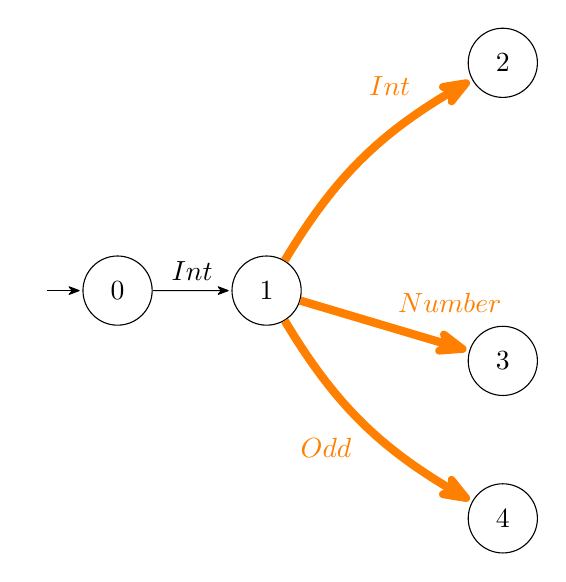
\begin{tikzpicture}[automaton, auto]
  \node[state,initial,rounded rectangle] (0) {$0$};
  \node[state,rounded rectangle] (1) [right=10mm of 0] {$1$};
  \node[state,rounded rectangle] (2) [above right=20mm and 30mm of 1] {$2$};
  \node[state,rounded rectangle] (3) [below right=0mm and 30mm of 1] {$3$};
  \node[state,rounded rectangle] (4) [below right=20mm and 30mm of 1] {$4$};
  \path[->] (0) edge node {$Int$} (1);
  \path[->] (1) edge[orange, line width=3pt, bend left=15]  node[pos=.8] {$Int$} (2);
  \path[->] (1) edge[orange, line width=3pt] node {$Number$} (3);
  \path[->] (1) edge[orange, line width=3pt, bend right=15] node[swap] {$Odd$} (4);
\end{tikzpicture}
\end{document}
